\documentclass[12pt,english]{beamer}
\usetheme{Rochester}
\graphicspath{{/home/raymond/report/Presentation_2/figures/}}
\DeclareGraphicsExtensions{.pdf,.jpg,.jpeg,.png}


\title{Contact Force Estimation for Robotic Assembly using Motor Currents/Torques}
\author{Raymond Djajalaksana, Fransisco Suarez, Quang-Cuong Pham}
\date{\today}

\begin{document}
  \frame{\titlepage}
  
  \begin{frame}
    \frametitle{Outline}
    \tableofcontents
  \end{frame}
    
  \section{Introduction}  
  \begin{frame}
    \frametitle{Introduction}
    \begin{itemize}
      \item To handle uncertainites and to adapt with dynamic environment, contact detection is essential for assembly arm. This requires the ability of the arm to estimate the contact force.
      \item F/T sensor will be a good way to solve this problem, though it has some limitations.
      \item Limitations of F/T sensor :
      \begin{itemize}
        \item expensive
        \item Requires mechanical integration
      \end{itemize}
    \end{itemize}
  \end{frame}
  
  \begin{frame}
    \frametitle{Introduction}
    \begin{itemize}
      \item Alternative ways to estimate the contact forces have been researched in early decades.
      \item Some approaches to estimate contact forces:
      \begin{itemize}
        \item detune the low-level joint position control loop
        \item generalized momentum with Kalman filter
        \item Bayesian approach
      \end{itemize}
      \item All approaches are rooted from robot dynamic equation.
    \end{itemize}
  \end{frame}
  
%----------------------------------------------------------------------------------------
  \section{Model Estimation}
  \begin{frame}
    \frametitle{Model Estimation}
    \begin{itemize}
      \item Robot dynamic equations:
      \begin{align}
        \tau_{mot} &= \tau_{dyn} + \tau_{ext} + \tau_{friction}\\
        \tau_{dyn} &= H\left(q\right)\ddot{q} + C\left(\dot{q} , q \right)\dot{q} + G\left(q \right)\\
        \tau_{ext} &= J^{T} F_{ext}\\
        \tau_{mot} &= K_{m} I_{mot}
      \end{align}
    \end{itemize}
  \end{frame}
  
  \begin{frame}
    \frametitle{Model Estimation}
    \begin{itemize}
      \item Simple static friction (viscous + coulomb) model:
      \begin{equation}
        \tau_{friction} = K_{c} sign\left(\dot{q}\right) + K_{v} \dot{q}
      \end{equation}
      \item Simple dynamic friction (Dahl) model:
      \begin{align}
        \dot{z} &= \dot{q} - \frac{\left|\dot{q}\right|}{F_{c}} \sigma z \\
        \tau_{friction} &= \sigma z
      \end{align}
    \end{itemize}
  \end{frame}
  
  \begin{frame}
    \frametitle{Model Estimation}
    \begin{itemize}
      \item Dahl friction diagram:
      \begin{figure}
        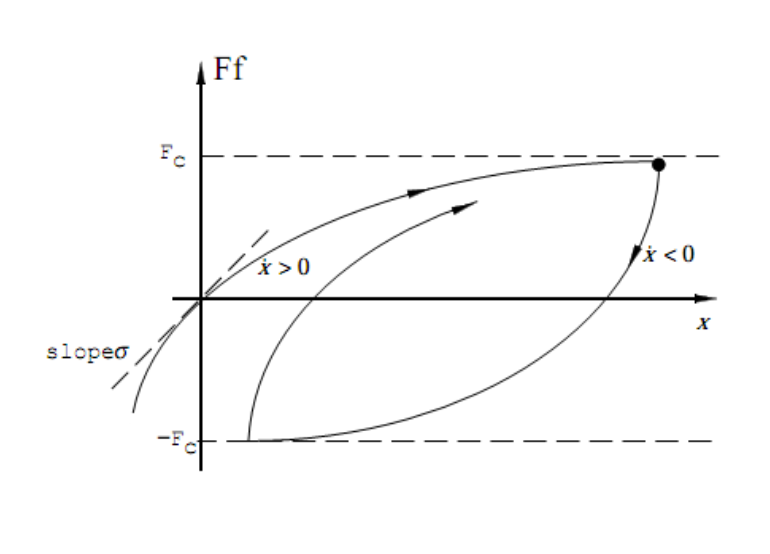
\includegraphics[width = 0.8\textwidth]{Dahl} \,
      \end{figure}
    \end{itemize}
  \end{frame}
  
%----------------------------------------------------------------------------------------
  \section{Setup}
  \begin{frame}
    \frametitle{Setup}
    \framesubtitle{Experimental Setup}
    Two types of experiments:
    \begin{itemize}
    \item First experiments (for joint 1,2,3, and 5) :
      \begin{itemize}
        \item home $\rightarrow$ pre-contact point $\rightarrow$ contact $\rightarrow$ sinusoidal motion
      \end{itemize}
    \item Second experiments (for joint 4 and 6) :
      \begin{itemize}
        \item home $\rightarrow$ stationary point $\rightarrow$ force is introduced to robot
      \end{itemize}
    \end{itemize}
  \end{frame}
  
  \begin{frame}
    \frametitle{Setup}
    \framesubtitle{Experimental Setup}
    First type of experiment:
    \begin{center}
      \href{run:exp_1.ogv}{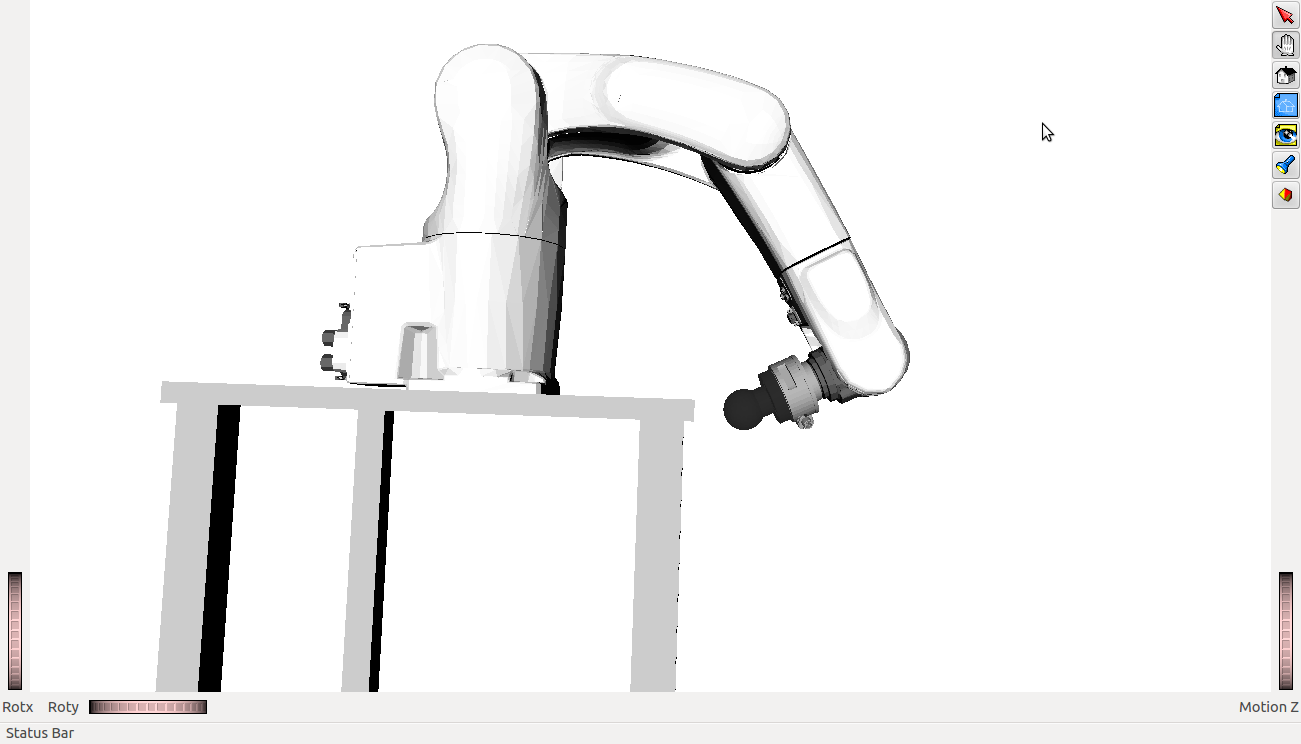
\includegraphics[width = 0.4\textwidth]{fig01}}
      \href{run:exp_2.ogv}{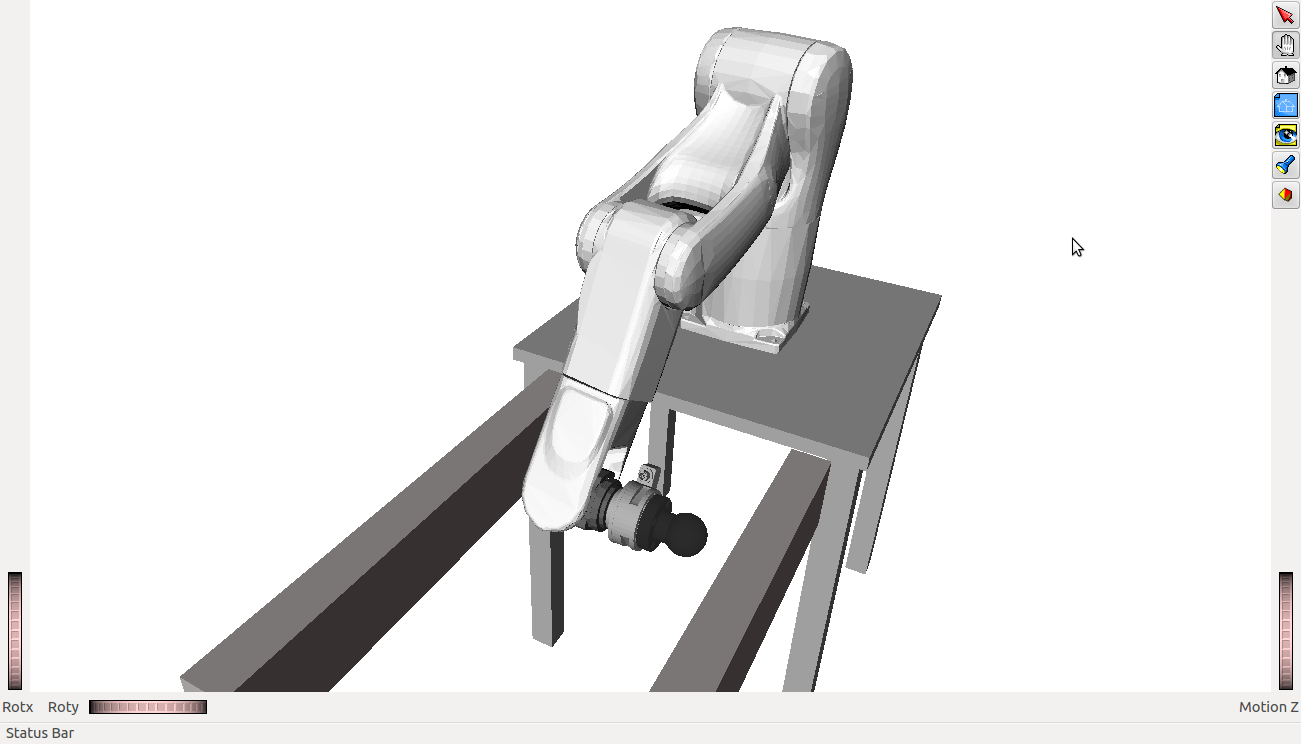
\includegraphics[width = 0.4\textwidth]{fig18}}
    \end{center}
  \end{frame}
  
  \begin{frame}
    \frametitle{Setup}
    \framesubtitle{Experimental Setup}
    Second type of experiment:
    \begin{center}
      \href{run:exp_3.ogv}{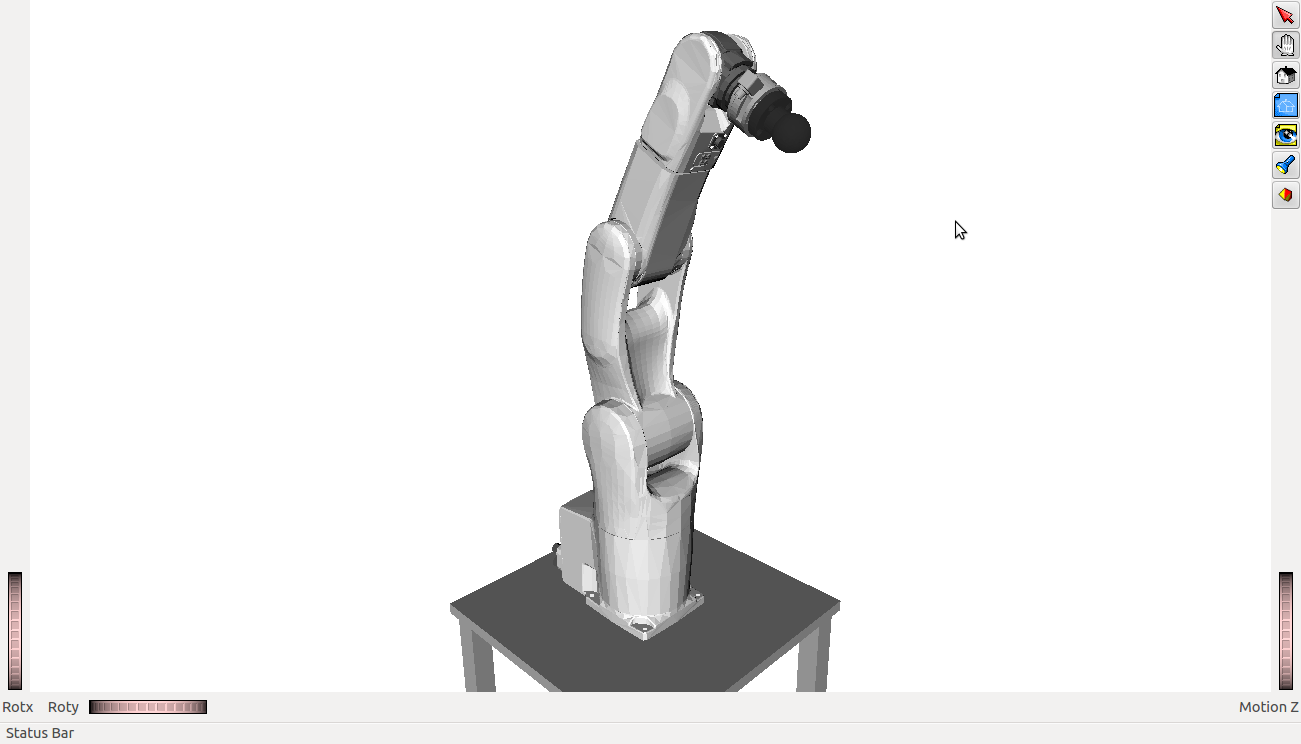
\includegraphics[width = 0.6\textwidth]{fig03}}
    \end{center}
  \end{frame}
  
  \begin{frame}
    \frametitle{Setup}
    \framesubtitle{Motor Currents Reading}
    \begin{itemize}
      \item Problem : Denso arm only gives absolute value of the motor currents. Needs a way to know the sign of motor currents.
      \begin{figure}
        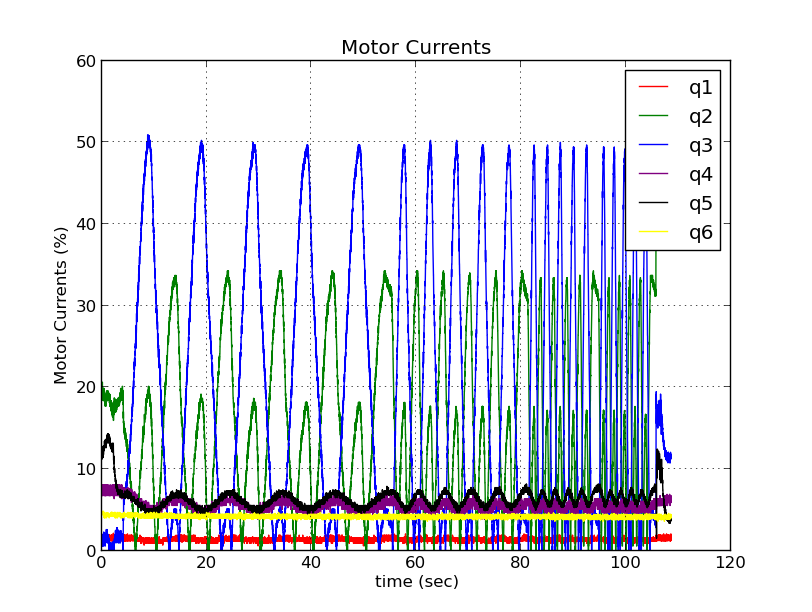
\includegraphics[scale=0.35]{fig04}
      \end{figure}
    \end{itemize}
  \end{frame}  
  
  \begin{frame}
    \frametitle{Setup}
    \framesubtitle{Motor Currents Reading}
    \begin{itemize}
      \item Some approaches to fix this problem:
      \begin{itemize}
        \item Use sign of $\tau_{dyn}$ to determine motor current sign.
        \item Use sign of $\Delta \tau_{dyn}$ value to determine motor current sign.
        \item Use sign of motor torques to give motor current sign.
      \end{itemize}
    \end{itemize}
  \end{frame}  
  
  \begin{frame}
    \frametitle{Setup}
    \framesubtitle{Motor Currents Reading}
    \begin{itemize}
      \item After implementing the third method.
      \begin{figure}
        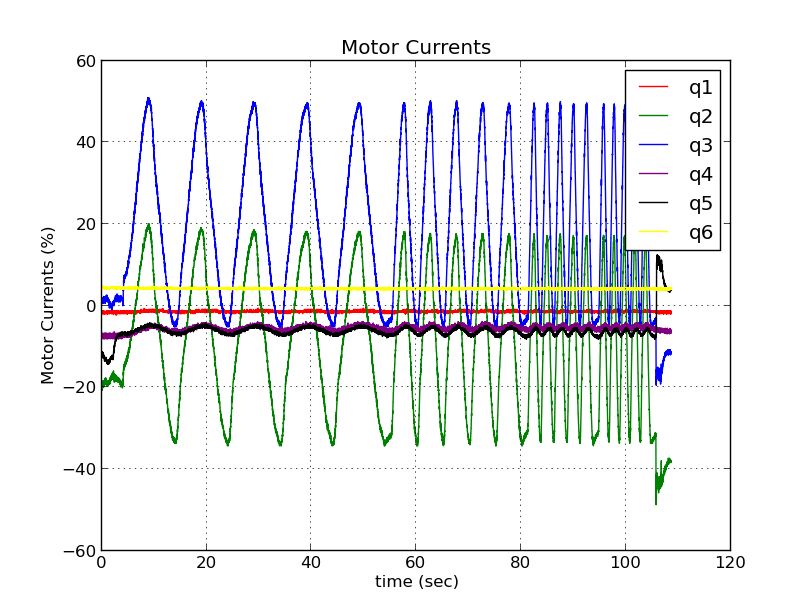
\includegraphics[scale=0.4]{fig05}
      \end{figure}
    \end{itemize}
  \end{frame}  

%----------------------------------------------------------------------------------------  
  \section{Results}
  \begin{frame}
    \frametitle{Results}
    \framesubtitle{Preliminary Results}
    \begin{itemize}
      \item First type of experiment :
      \begin{columns}
        \column{0.5\textwidth}
        \begin{figure}
          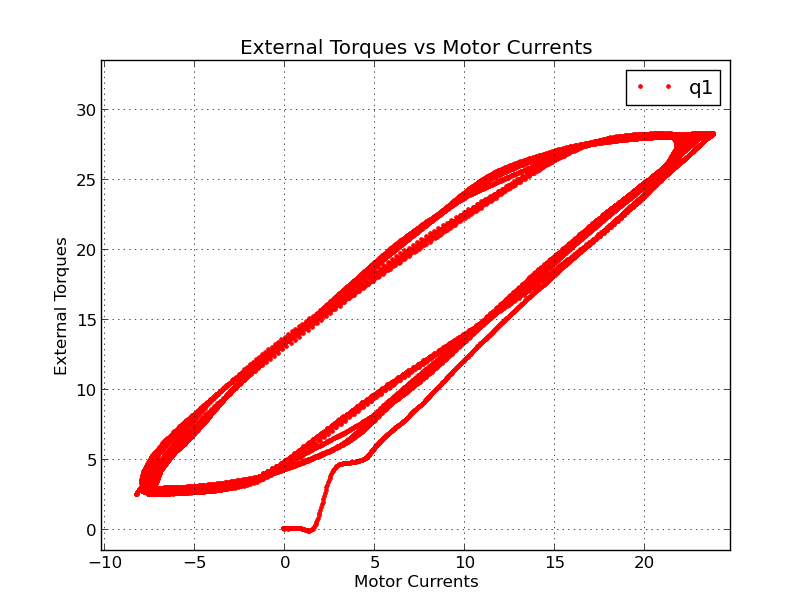
\includegraphics[height = 0.5\textwidth]{fig06} \,
          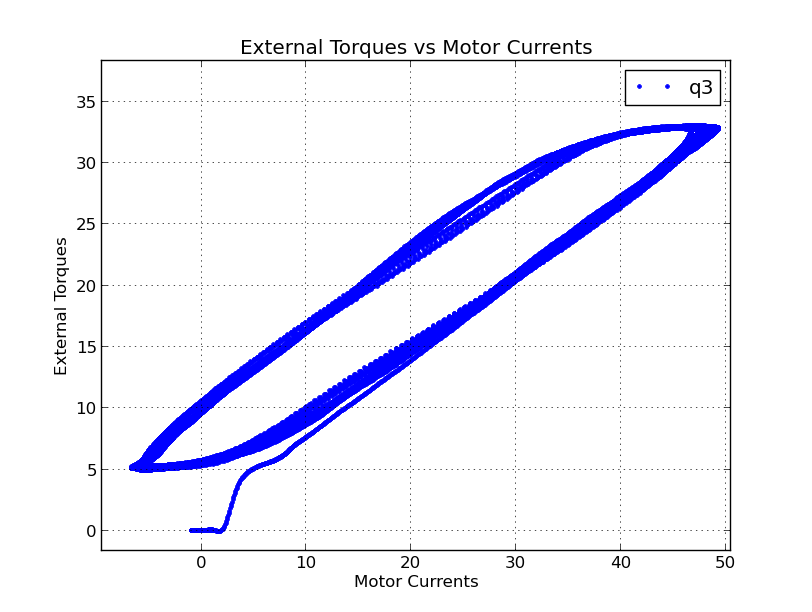
\includegraphics[height = 0.5\textwidth]{fig08} \,
        \end{figure}
        \column{0.5\textwidth}
        \begin{figure}
          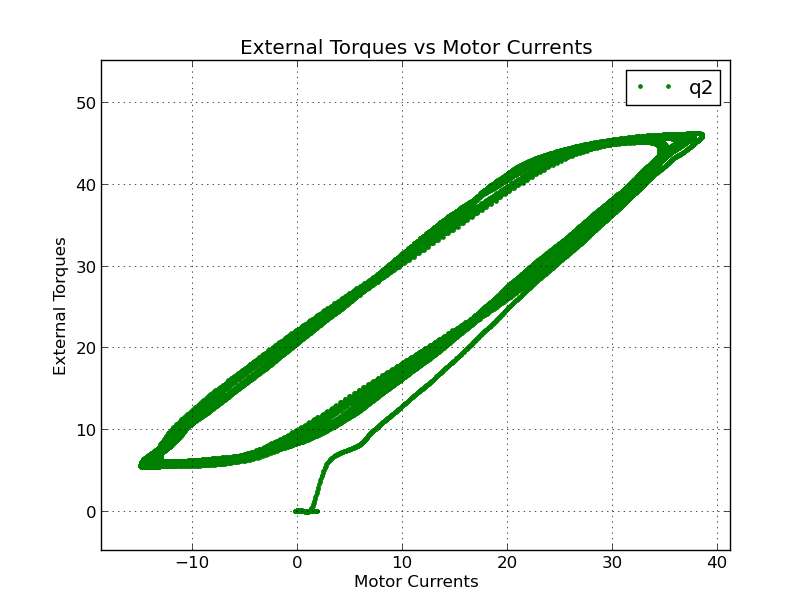
\includegraphics[height = 0.5\textwidth]{fig07} \,
          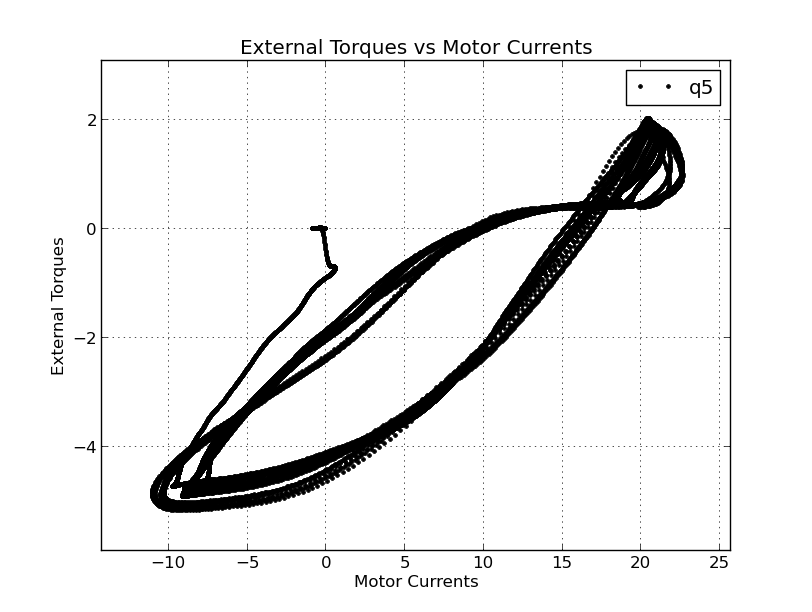
\includegraphics[height = 0.5\textwidth]{fig10} \,
        \end{figure}
      \end{columns}
    \end{itemize}
  \end{frame}
  
  \begin{frame}
    \frametitle{Results}
    \framesubtitle{Preliminary Results}
    \begin{itemize}
      \item Second type of experiment :
      \begin{columns}
        \column{0.6\textwidth}
        \begin{figure}
          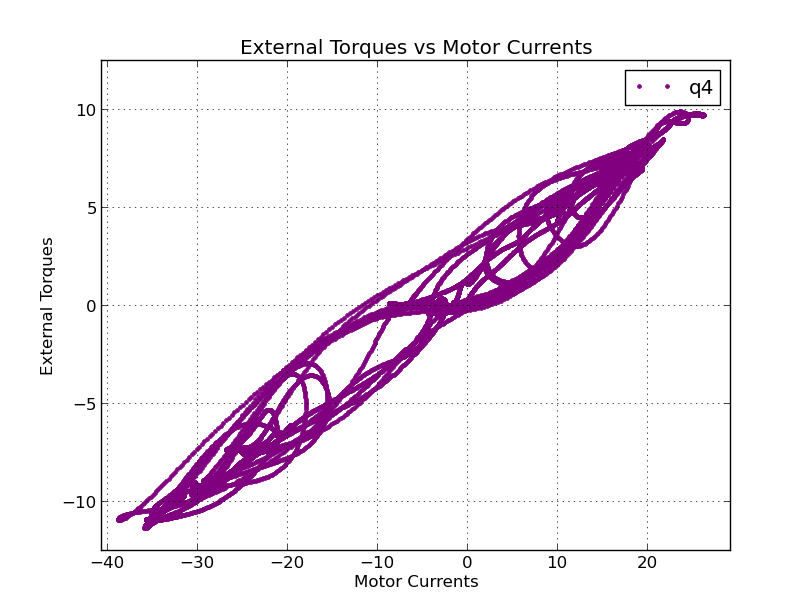
\includegraphics[width = \textwidth]{fig09} \,
        \end{figure}
        \column{0.6\textwidth}
        \begin{figure}
          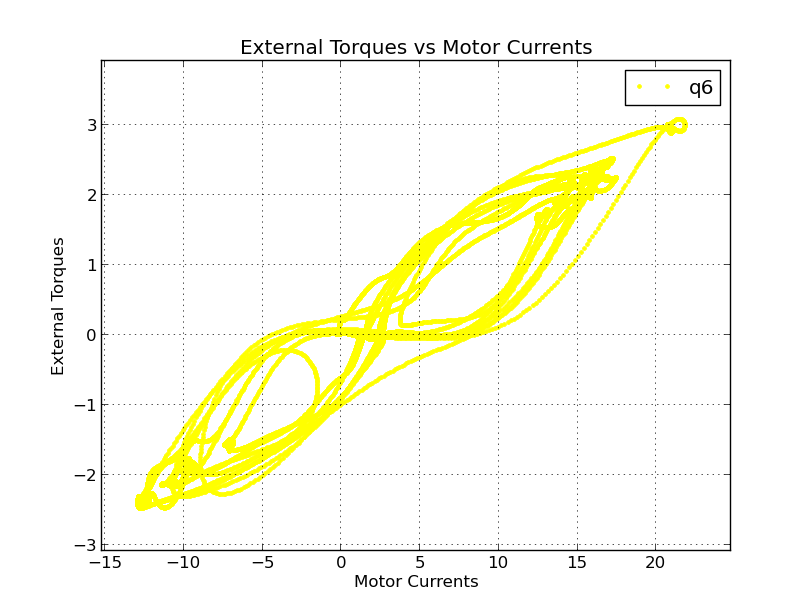
\includegraphics[width = \textwidth]{fig11} \,
        \end{figure}
      \end{columns}
    \end{itemize}
  \end{frame}
  
  \begin{frame}
    \frametitle{Results}
    \framesubtitle{Model Identification}
    \begin{itemize}
    \item Modified equation to be identified :
    \begin{equation}
      J^{T} \Delta F_{ext} = K_{m} sign\left(\tau_{mot}\right) \Delta I_{mot} - \Delta \tau_{friction} + C
    \end{equation}
    \item Identification is done by optimizing the model parameters so it will match into the data. The optimization is done using Nelder-mead method.
    \end{itemize}
  \end{frame}
  
  \begin{frame}
    \frametitle{Results}
    \framesubtitle{Model Identification}
    \begin{itemize}
    \item Static friction model will be used as it is.
    \item Modification of Dahl model for optimization :
    \begin{align}
      \dot{z} &= p_{2 }\dot{\tau_{mot}} - \left|\dot{\tau_{mot}}\right| p_{3} z \\
      \tau_{friction} &= p_{1} z
    \end{align}
    \item Optimization: 4 parameters for static friction. 6 parameters for dynamic friction.
    \end{itemize}
  \end{frame}
  
  
  \begin{frame}
    \frametitle{Results}
    \framesubtitle{Model Identification}
    Results of optimization:
    \begin{center}
      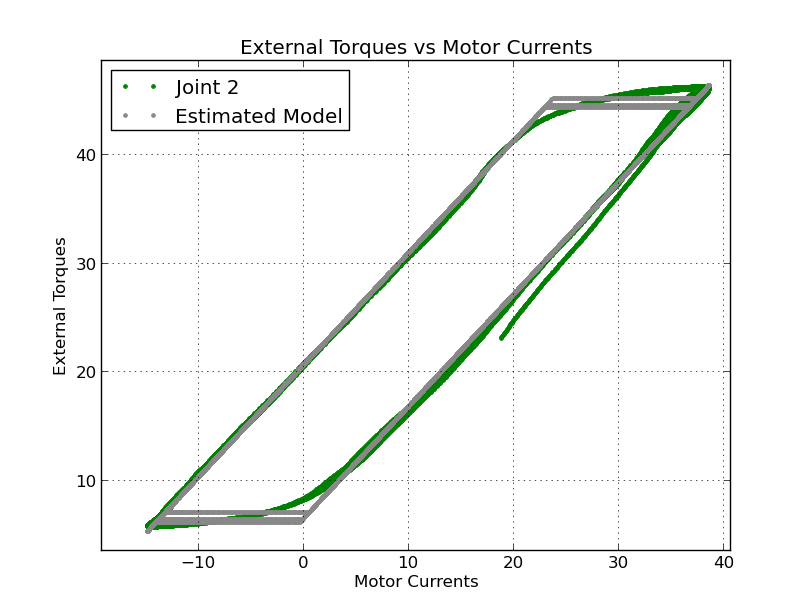
\includegraphics[width = 0.55\textwidth]{fig12}
      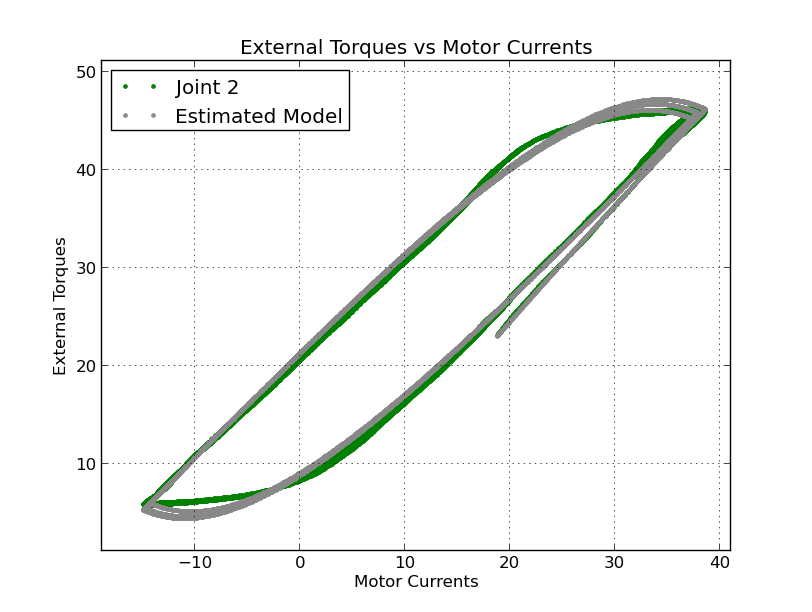
\includegraphics[width = 0.55\textwidth]{fig13}
    \end{center}
  \end{frame}
  
  
  \begin{frame}
    \frametitle{Results}
    \framesubtitle{Validation}
    Contact force estimation
    \begin{columns}
      \column{0.6\textwidth}
      \centering
        \begin{figure}
          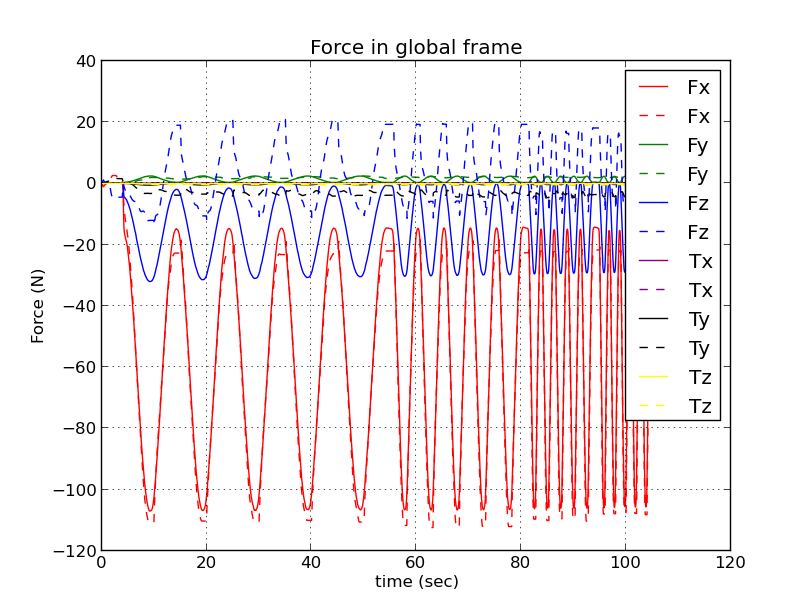
\includegraphics[width = \textwidth]{fig14}
        \end{figure}
        Static friction model
      \column{0.6\textwidth}
      \centering
        \begin{figure}
          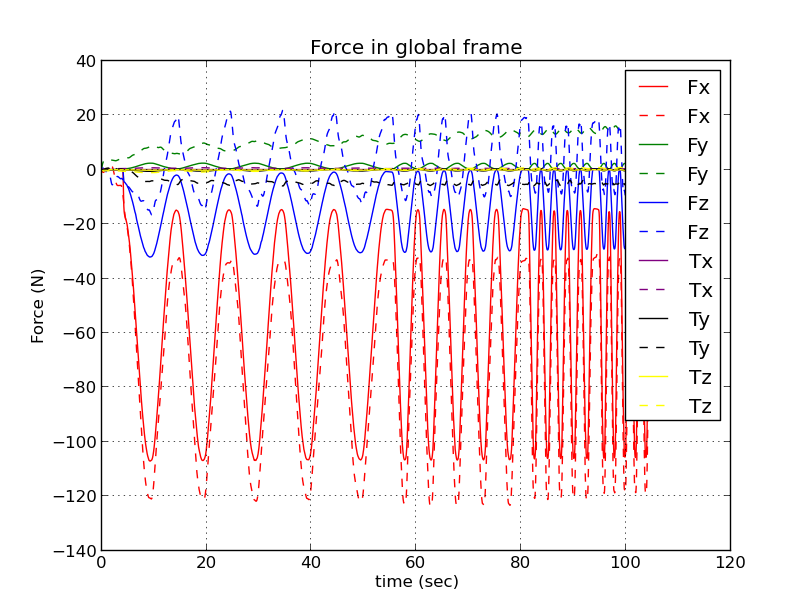
\includegraphics[width = \textwidth]{fig15}
        \end{figure}
        Dynamic friction model
    \end{columns}
  \end{frame}

  \begin{frame}
    \frametitle{Results}
    \framesubtitle{Validation}
    External joint torque estimation
    \begin{columns}
      \column{0.6\textwidth}
      \centering
        \begin{figure}
          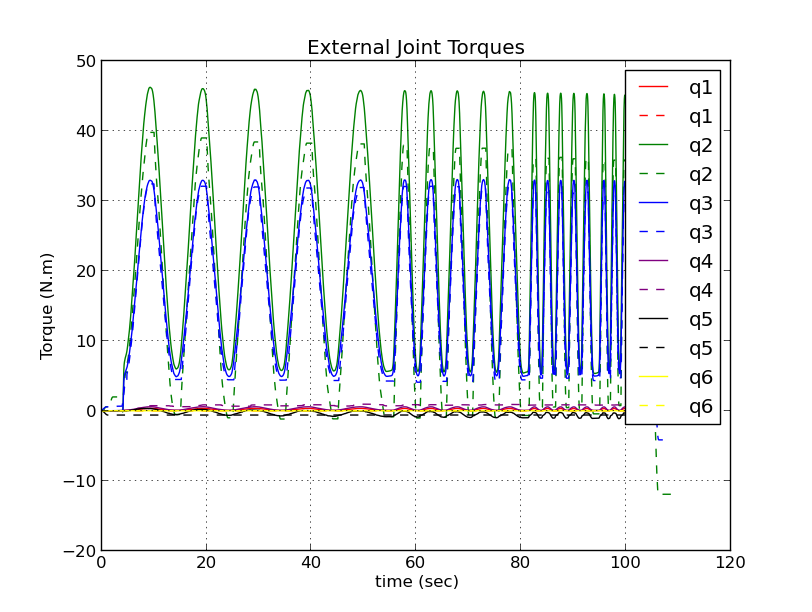
\includegraphics[width = \textwidth]{fig16}
        \end{figure}
        Static friction model
      \column{0.6\textwidth}
      \centering
        \begin{figure}
          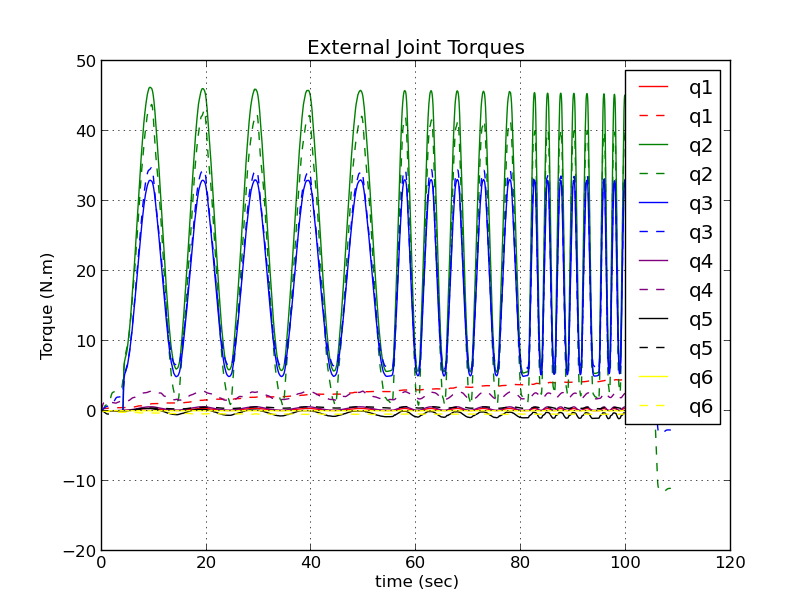
\includegraphics[width = \textwidth]{fig17}
        \end{figure}
        Dynamic friction model
    \end{columns}
  \end{frame}
  
  \begin{frame}
    \frametitle{Results}
    \framesubtitle{Validation}
    \begin{columns}
      \column{0.5\textwidth}
        Static friction model
        \begin{itemize}
          \item quantitatively less accurate for second and thrid joint torque estimation.
          \item discrete pattern.
        \end{itemize}
      \column{0.5\textwidth}
        Dynamic friction model
        \begin{itemize}
          \item quantitatively more accurate for second and thrid joint torque estimation.
          \item continuous profile.
          \item results are drifted.
          \item difficulty to estimate first initial internal state.
        \end{itemize}
    \end{columns}
  \end{frame}
%----------------------------------------------------------------------------------------
  \section{Future Works} 
  \begin{frame}
    \frametitle{Future Works}
    \begin{itemize}
      \item Test the results in real time operation.
      \item Start controlling the robot for assembly task.
    \end{itemize}
  \end{frame}
\end{document}


